%!TEX root = ../erweiterte_sachkunde.tex
\chapter{Anatomie und Physiologie des Hundes}


\section{Allgemeiner Aufbau und anatomische Lage}
        \begin{figure}[ht]
        \centering
        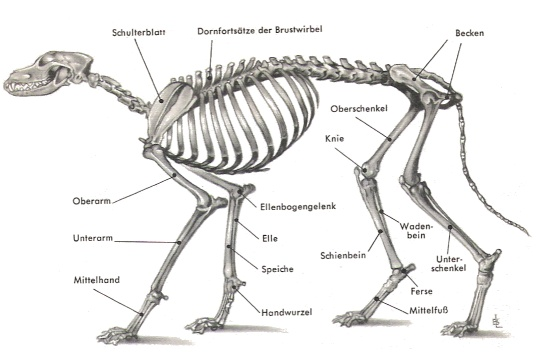
\includegraphics[width=1.0\textwidth]{./bilder/anatomie1.jpg}
        \caption{Skelett \label{overflow}}
        \end{figure}

        \begin{figure}[ht]
        \centering
        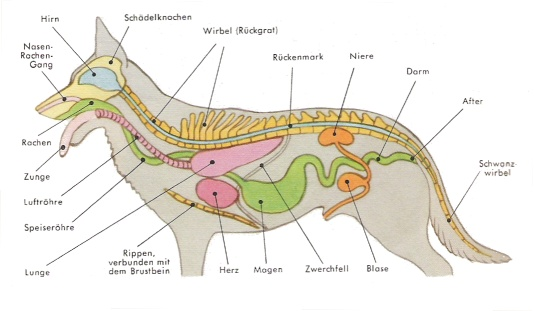
\includegraphics[width=1.0\textwidth]{./bilder/anatomie2.jpg}
        \caption{Organe \label{overflow}}
        \end{figure}

    \subsection{Bewegungsapparat mit Knochen, Muskeln und Gelenken}


\section{Einzelheiten}

\section{Ausgewählte Erkrankungen}

\section{Impfungen}